\chapter{Результаты} \label{chapt3}


\section{Незвешенные графы} \label{sect3_1}

\subsection{$\varepsilon$-графы} \label{sect3_1_1}

Результаты экспериментов представлены на графиках. Использовались графы на 250 вершинах.
Во всех случаях по оси $x$ отложены значения параметра семейства. Для удобства все параметры были отнормированы на отрезок $[0,1]$ с помощью дробно-линейного преобразования. В случае коэффициентов корреляции правый рисунок показывает увеличенную область больших значений коэффициента ($>0.8$).

\begin{figure}[h]
  \begin{minipage}[h]{0.49\linewidth}
    \center{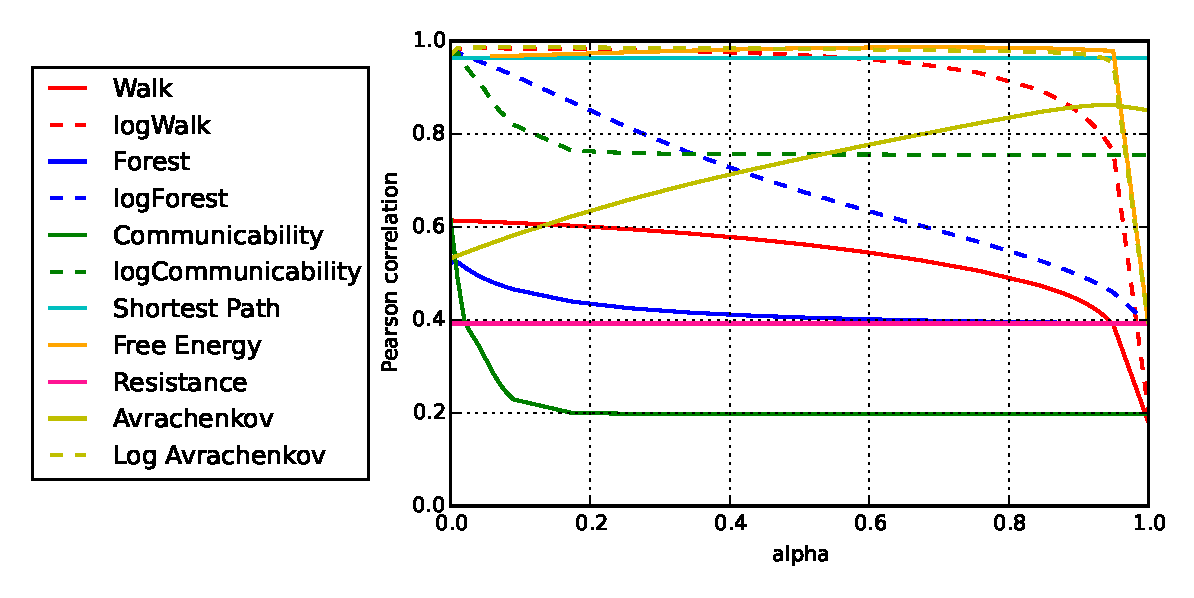
\includegraphics[width=0.95\linewidth]{correlations_eps}}
  \end{minipage}
  \hfill
  \begin{minipage}[h]{0.49\linewidth}
    \center{\includegraphics[width=0.95\linewidth]{correlations_zoom_eps}}
  \end{minipage}

  \caption{Корреляции Пирсона для $\varepsilon$-графов}
  \label{img:eps_graphs}  
\end{figure}

%===========================================
\begin{figure}[h]
  \begin{minipage}[h]{0.49\linewidth}
    \center{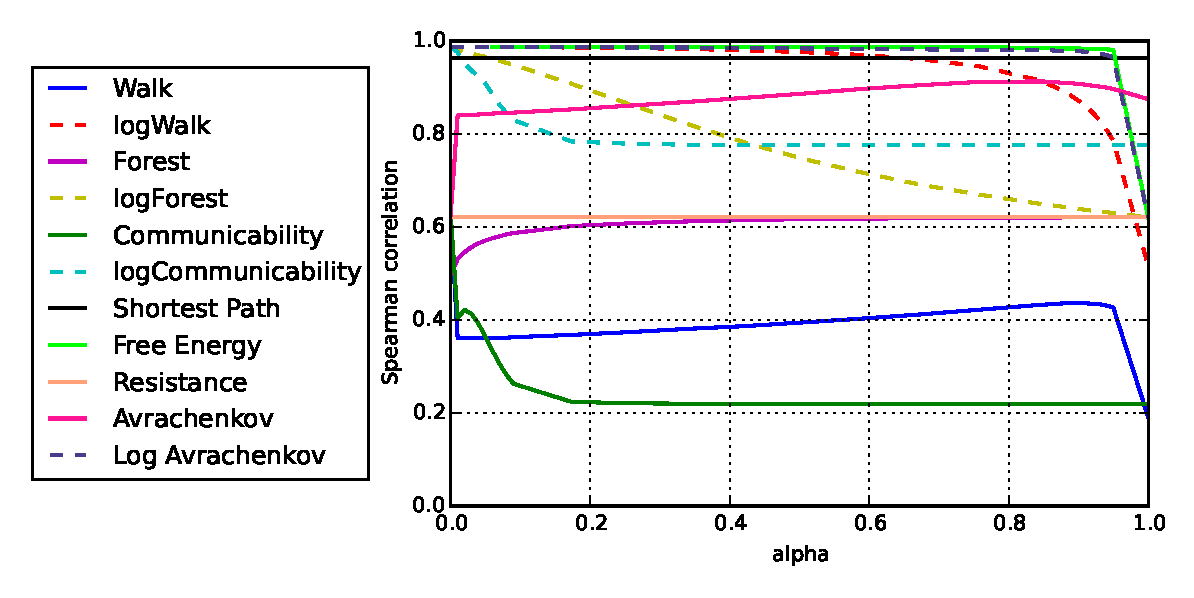
\includegraphics[width=0.95\linewidth]{sp_correlations_eps}}
  \end{minipage}
  \hfill
  \begin{minipage}[h]{0.49\linewidth}
    \center{\includegraphics[width=0.95\linewidth]{sp_correlations_zoom_eps}}
  \end{minipage}

  \caption{Корреляции Спирмена для $\varepsilon$-графов}
  \label{img:eps_graphs_sp}  
\end{figure}

%===========================================

\begin{figure}[h]
  \begin{minipage}[h]{0.49\linewidth}
    \center{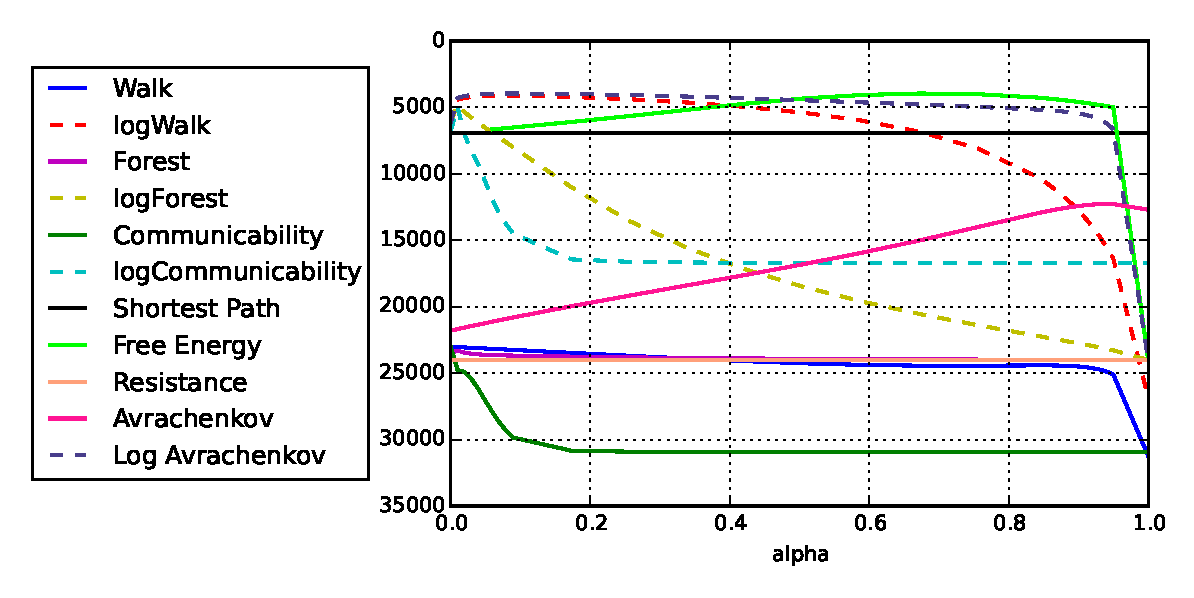
\includegraphics[width=0.95\linewidth]{1norm_eps}}
  \end{minipage}
  \hfill
  \begin{minipage}[h]{0.49\linewidth}
    \center{\includegraphics[width=0.95\linewidth]{2norm_eps}}
  \end{minipage}

  \caption{Матричные нормы для $\varepsilon$-графов: слева - 1-норма, справа - 2-норма}
  \label{img:eps_graphs_norm}  
\end{figure}

%===========================================
\newpage
 Значения параметров, при которых метрики лучше всего приближают евклидово расстояние, и значение коэффициента корреляции Пирсона для данных параметров, приведены в таблице:
 
\begin{table} [!htbp]
  \centering
  \parbox{15cm}{\caption{Параметры метрик для $\varepsilon$-графов}\label{Ts0Sib}}
%  \begin{center}
  \begin{tabular}{| p{6cm} || p{2.5cm} | p{2.5cm}l |}
  \hline
  \hline
  Метрика   & \centering Значение параметра из $[0,1]$ & \centering  Корреляция Пирсона& \\
  \hline
  Walk &\centering  0.35   &\centering  0.613   &  \\
  \hline
  Log Walk  &\centering  0.15   &\centering  0.984    &  \\
  \hline
  Forest &\centering  1.0   &\centering  0.525   &  \\
  \hline
  Log Forest &\centering  0.005   &\centering  0.975   &   \\
  \hline
  Communicability &\centering  0.02   &\centering  0.613    & \\
  \hline
  Log Communicability &\centering  0.01   &\centering  0.975 &  \\
  \hline
  Shortest Path &\centering  не зависит   &\centering  0.964 & \\
  \hline
  Resistance &\centering  не зависит   &\centering  0.392     & \\
  \hline
  Free Energy &\centering  0.7   &\centering  0.986      & \\
  \hline
  Avrachenkov &\centering  0.87   &\centering  0.863    &\\
  \hline
  Log Avrachenkov &\centering  0.08   &\centering  0.986  &  \\
  \hline
  \hline
  \end{tabular}
%  \end{center}
\end{table}


\clearpage
%===========================================
\subsection{Симметричные графы ближайших соседей} \label{sect3_1_2}

Результаты экспериментов представлены на графиках. Использовались графы на 250 вершинах, параметр $k = 8$. 
Во всех случаях по оси $x$ отложены значения параметра семейства. Для удобства все параметры были отнормированы на отрезок $[0,1]$ с помощью дробно-линейного преобразования. В случае коэффициентов корреляции правый рисунок показывает увеличенную область больших значений коэффициента ($>0.8$).

\begin{figure}[h]
  \begin{minipage}[h]{0.49\linewidth}
    \center{\includegraphics[width=0.95\linewidth]{correlations_sym}}
  \end{minipage}
  \hfill
  \begin{minipage}[h]{0.49\linewidth}
    \center{\includegraphics[width=0.95\linewidth]{correlations_zoom_sym}}
  \end{minipage}

  \caption{Корреляции Пирсона для симметричных графов ближайших соседей}
  \label{img:sym_graphs}  
\end{figure}

%===========================================
\begin{figure}[h]
  \begin{minipage}[h]{0.49\linewidth}
    \center{\includegraphics[width=0.95\linewidth]{sp_correlations_sym}}
  \end{minipage}
  \hfill
  \begin{minipage}[h]{0.49\linewidth}
    \center{\includegraphics[width=0.95\linewidth]{sp_correlations_zoom_sym}}
  \end{minipage}

  \caption{Корреляции Спирмена для симметричных графов ближайших соседей}
  \label{img:sym_graphs_sp}  
\end{figure}

%===========================================

\begin{figure}[h]
  \begin{minipage}[h]{0.49\linewidth}
    \center{\includegraphics[width=0.95\linewidth]{1norm_sym}}
  \end{minipage}
  \hfill
  \begin{minipage}[h]{0.49\linewidth}
    \center{\includegraphics[width=0.95\linewidth]{2norm_sym}}
  \end{minipage}

  \caption{Матричные нормы для симметричных графов ближайших соседей: слева - 1-норма, справа - 2-норма}
  \label{img:sym_graphs_norm}  
\end{figure}

%===========================================

%===========================================

\newpage
 Значения параметров, при которых метрики лучше всего приближают евклидово расстояние, и значение коэффициента корреляции Пирсона для данных параметров, приведены в таблице:

\begin{table} [!htbp]
  \centering
  \parbox{15cm}{\caption{Параметры метрик для симметричных графов ближайших соседей}\label{Ts0Sib}}
%  \begin{center}
  \begin{tabular}{| p{6cm} || p{2.5cm} | p{2.5cm}l |}
  \hline
  \hline
  Метрика   & \centering Значение параметра из $[0,1]$ & \centering  Корреляция Пирсона & \\
  \hline
  Walk &\centering  0.87   &\centering  0.432   &  \\
  \hline
  Log Walk  &\centering  0.18   &\centering  0.919    &  \\
  \hline
  Forest &\centering  1.0   &\centering  0.869    &  \\
  \hline
  Log Forest &\centering  0.005   &\centering  0.919   &   \\
  \hline
  Communicability &\centering  0.3   &\centering  0.416    & \\
  \hline
  Log Communicability &\centering  0.01   &\centering  0.918 &  \\
  \hline
  Shortest Path &\centering  не зависит   &\centering  0.912     & \\
  \hline
  Resistance &\centering  не зависит   &\centering  0.869     & \\
  \hline
  Free Energy &\centering  0.85   &\centering  0.920      & \\
  \hline
  Avrachenkov &\centering  0.95   &\centering  0.813    &\\
  \hline
  Log Avrachenkov &\centering  1.0   &\centering  0.920  &  \\
  \hline
  \hline
  \end{tabular}
%  \end{center}
\end{table}

%=================================

\clearpage

\subsection{Графы взаимных ближайших соседей} \label{subsect3_1_3}

Результаты экспериментов представлены на графиках. Использовались графы на 250 вершинах, параметр $k = 12$. 
Во всех случаях по оси $x$ отложены значения параметра семейства. Для удобства все параметры были отнормированы на отрезок $[0,1]$ с помощью дробно-линейного преобразования. В случае коэффициентов корреляции правый рисунок показывает увеличенную область больших значений коэффициента ($>0.8$).

%===========================================
\begin{figure}[!htbp]
  \begin{minipage}[h]{0.49\linewidth}
    \center{\includegraphics[width=0.95\linewidth]{correlations_mut}}
  \end{minipage}
  \hfill
  \begin{minipage}[h]{0.49\linewidth}
    \center{\includegraphics[width=0.95\linewidth]{correlations_zoom_mut}}
  \end{minipage}

  \caption{Корреляции Пирсона для графов взаимных ближайших соседей}
  \label{img:mut_graphs}  
\end{figure}

%===========================================
\begin{figure}[h]
  \begin{minipage}[h]{0.49\linewidth}
    \center{\includegraphics[width=0.95\linewidth]{sp_correlations_mut}}
  \end{minipage}
  \hfill
  \begin{minipage}[h]{0.49\linewidth}
    \center{\includegraphics[width=0.95\linewidth]{sp_correlations_zoom_mut}}
  \end{minipage}

  \caption{Корреляции Спирмена для графов взаимных ближайших соседей}
  \label{img:mut_graphs_sp}  
\end{figure}

%===========================================

\begin{figure}[h]
  \begin{minipage}[h]{0.49\linewidth}
    \center{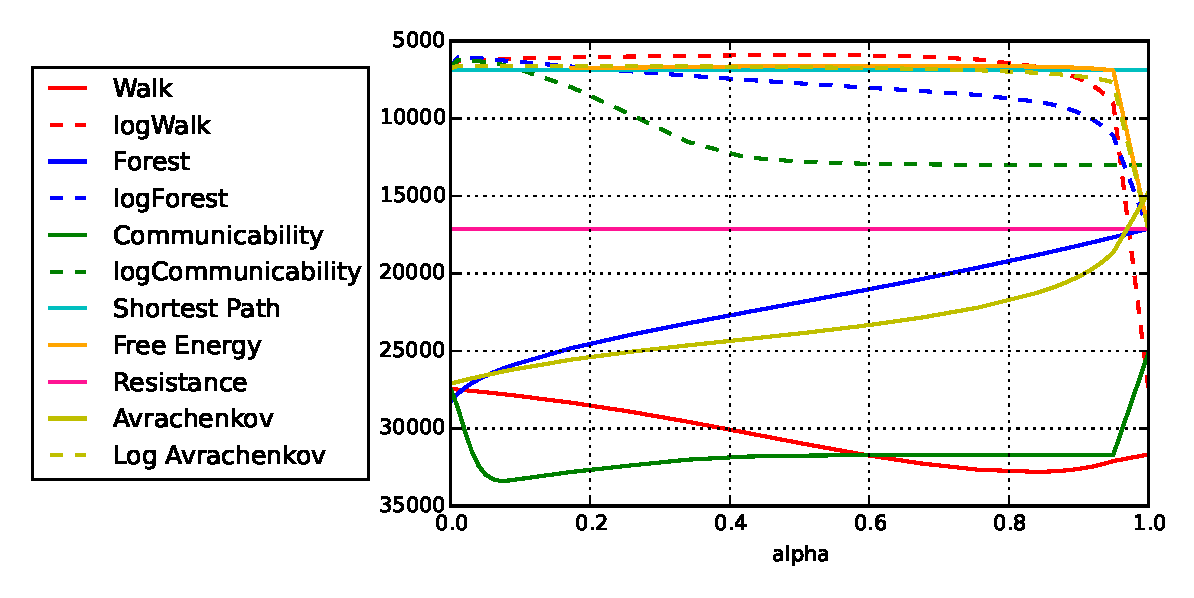
\includegraphics[width=0.95\linewidth]{1norm_mut}}
  \end{minipage}
  \hfill
  \begin{minipage}[h]{0.49\linewidth}
    \center{\includegraphics[width=0.95\linewidth]{2norm_mut}}
  \end{minipage}

  \caption{Матричные нормы для графов взаимных ближайших соседей: слева - 1-норма, справа - 2-норма}
  \label{img:mut_graphs_norm}  
\end{figure}

%===========================================
\newpage
 Значения параметров, при которых метрики лучше всего приближают евклидово расстояние, и значение коэффициента корреляции Пирсона для данных параметров, приведены в таблице:
 
\begin{table} [!htbp]
  \centering
  \parbox{15cm}{\caption{Параметры метрик для графов взаимных ближайших соседей}\label{Ts0Sib}}
%  \begin{center}
  \begin{tabular}{| p{6cm} || p{2.5cm} | p{2.5cm}l |}
  \hline
  \hline
  Метрика   & \centering Значение параметра из $[0,1]$ & \centering  Корреляция Пирсона & \\
  \hline
  Walk &\centering  0.01  &\centering  0.319   &  \\
  \hline
  Log Walk  &\centering  0.67   &\centering  0.963    &  \\
  \hline
  Forest &\centering  1.0   &\centering  0.669    &  \\
  \hline
  Log Forest &\centering  0.015   &\centering  0.961   &   \\
  \hline
  Communicability &\centering  0.9   &\centering  0.321    & \\
  \hline
  Log Communicability &\centering  0.025   &\centering  0.960 &  \\
  \hline
  Shortest Path &\centering  не зависит   &\centering  0.954     & \\
  \hline
  Resistance &\centering  не зависит   &\centering  0.669     & \\
  \hline
  Free Energy &\centering  0.58   &\centering  0.956      & \\
  \hline
  Avrachenkov &\centering  0.95  &\centering  0.680    &\\
  \hline
  Log Avrachenkov &\centering  0.035   &\centering  0.956  &  \\
  \hline
  \hline
  \end{tabular}
%  \end{center}
\end{table}

%\newpage
%============================================================================================================================
\clearpage

\section{Взвешенные графы} \label{sect3_2}

Результаты экспериментов представлены на графиках. Использовались графы на 250 вершинах, параметр $\sigma = 5$.
Во всех случаях по оси $x$ отложены значения параметра семейства. Для удобства все параметры были отнормированы на отрезок $[0,1]$ с помощью дробно-линейного преобразования. В случае коэффициентов корреляции правый рисунок показывает увеличенную область больших значений коэффициента ($>0.8$).

\begin{figure}[h]
  \begin{minipage}[h]{0.49\linewidth}
    \center{\includegraphics[width=0.95\linewidth]{correlations_wei}}
  \end{minipage}
  \hfill
  \begin{minipage}[h]{0.49\linewidth}
    \center{\includegraphics[width=0.95\linewidth]{correlations_zoom_wei}}
  \end{minipage}

  \caption{Корреляции Пирсона для гауссовских графов}
  \label{img:wei_graphs}  
\end{figure}

%===========================================
\begin{figure}[h]
  \begin{minipage}[h]{0.49\linewidth}
    \center{\includegraphics[width=0.95\linewidth]{correlations_sp_wei}}
  \end{minipage}
  \hfill
  \begin{minipage}[h]{0.49\linewidth}
    \center{\includegraphics[width=0.95\linewidth]{correlations_sp_zoom_wei}}
  \end{minipage}

  \caption{Корреляции Спирмена для гауссовских графов}
  \label{img:wei_graphs_sp}  
\end{figure}

%===========================================

\begin{figure}[h]
  \begin{minipage}[h]{0.49\linewidth}
    \center{\includegraphics[width=0.95\linewidth]{1norm_wei}}
  \end{minipage}
  \hfill
  \begin{minipage}[h]{0.49\linewidth}
    \center{\includegraphics[width=0.95\linewidth]{2norm_wei}}
  \end{minipage}

  \caption{Матричные нормы для гауссовских графов: слева - 1-норма, справа - 2-норма}
  \label{img:wei_graphs_norm}  
\end{figure}

%===========================================

%===========================================

\newpage
 Значения параметров, при которых метрики лучше всего приближают евклидово расстояние, и значение коэффициента корреляции Пирсона для данных параметров, приведены в таблице:


\begin{table} [!htbp]
  \centering
  \parbox{15cm}{\caption{Параметры метрик для гауссовских графов}\label{Ts0Sib}}
%  \begin{center}
  \begin{tabular}{| p{6cm} || p{2.5cm} | p{2.5cm}l |}
  \hline
  \hline
  Метрика   & \centering Значение параметра из $[0,1]$ & \centering  Корреляция Пирсона & \\
  \hline
  Walk &\centering  0.87   &\centering  0.951   &  \\
  \hline
  Log Walk  &\centering  0.18   &\centering  0.986    &  \\
  \hline
  e-Walk &\centering  0.3   &\centering  0.915    & \\
  \hline
  Log e-Walk &\centering  0.01   &\centering  0.994 &  \\
  \hline
  Forest &\centering  1.0   &\centering  0.501    &  \\
  \hline
  Log Forest &\centering  0.005   &\centering  0.972   &   \\
  \hline  
  Shortest Path &\centering  не зависит   &\centering  0.995 & \\
  \hline
  Resistance &\centering  не зависит   &\centering  0.489     & \\
  \hline
  Free Energy &\centering  0.85   &\centering  0.995      & \\
  \hline
  Avrachenkov &\centering  0.95   &\centering  0.959    &\\
  \hline
  Log Avrachenkov &\centering  1.0   &\centering  0.992  &  \\
  \hline
  \hline
  \end{tabular}
%  \end{center}
\end{table}

%=================================
\section{Комментарии к результатам} \label{sect3_3} 

Данные графики были получены в результате усреднения по 50 экспериментам.

Максимумы на графиках незначительно меняют свое положение при изменении параметров графа до тех пор, пока он не начинает распадаться на кластеры, после чего значения коэффициентов корреляции в максимумах начинает уменьшаться.

Заметим, что в случае метрики Авраченкова представлены результаты только для $\sigma=1.0$, для других значений данного параметра зависимость от параметра аналогичная. Это связано с близостью степеней вершин в исследуемых графах.

В результате экспериментов для поиска оптимальных степеней выяснилось, что возведение элементов матрицы $D$ в степени, отличные от $1.0$, не улучшают качества приближения евклидового расстояния.

\clearpage